% Options for packages loaded elsewhere
\PassOptionsToPackage{unicode}{hyperref}
\PassOptionsToPackage{hyphens}{url}
%
\documentclass[
]{article}
\usepackage{amsmath,amssymb}
\usepackage{iftex}
\ifPDFTeX
  \usepackage[T1]{fontenc}
  \usepackage[utf8]{inputenc}
  \usepackage{textcomp} % provide euro and other symbols
\else % if luatex or xetex
  \usepackage{unicode-math} % this also loads fontspec
  \defaultfontfeatures{Scale=MatchLowercase}
  \defaultfontfeatures[\rmfamily]{Ligatures=TeX,Scale=1}
\fi
\usepackage{lmodern}
\ifPDFTeX\else
  % xetex/luatex font selection
\fi
% Use upquote if available, for straight quotes in verbatim environments
\IfFileExists{upquote.sty}{\usepackage{upquote}}{}
\IfFileExists{microtype.sty}{% use microtype if available
  \usepackage[]{microtype}
  \UseMicrotypeSet[protrusion]{basicmath} % disable protrusion for tt fonts
}{}
\makeatletter
\@ifundefined{KOMAClassName}{% if non-KOMA class
  \IfFileExists{parskip.sty}{%
    \usepackage{parskip}
  }{% else
    \setlength{\parindent}{0pt}
    \setlength{\parskip}{6pt plus 2pt minus 1pt}}
}{% if KOMA class
  \KOMAoptions{parskip=half}}
\makeatother
\usepackage{xcolor}
\usepackage[margin=1in]{geometry}
\usepackage{color}
\usepackage{fancyvrb}
\newcommand{\VerbBar}{|}
\newcommand{\VERB}{\Verb[commandchars=\\\{\}]}
\DefineVerbatimEnvironment{Highlighting}{Verbatim}{commandchars=\\\{\}}
% Add ',fontsize=\small' for more characters per line
\usepackage{framed}
\definecolor{shadecolor}{RGB}{248,248,248}
\newenvironment{Shaded}{\begin{snugshade}}{\end{snugshade}}
\newcommand{\AlertTok}[1]{\textcolor[rgb]{0.94,0.16,0.16}{#1}}
\newcommand{\AnnotationTok}[1]{\textcolor[rgb]{0.56,0.35,0.01}{\textbf{\textit{#1}}}}
\newcommand{\AttributeTok}[1]{\textcolor[rgb]{0.13,0.29,0.53}{#1}}
\newcommand{\BaseNTok}[1]{\textcolor[rgb]{0.00,0.00,0.81}{#1}}
\newcommand{\BuiltInTok}[1]{#1}
\newcommand{\CharTok}[1]{\textcolor[rgb]{0.31,0.60,0.02}{#1}}
\newcommand{\CommentTok}[1]{\textcolor[rgb]{0.56,0.35,0.01}{\textit{#1}}}
\newcommand{\CommentVarTok}[1]{\textcolor[rgb]{0.56,0.35,0.01}{\textbf{\textit{#1}}}}
\newcommand{\ConstantTok}[1]{\textcolor[rgb]{0.56,0.35,0.01}{#1}}
\newcommand{\ControlFlowTok}[1]{\textcolor[rgb]{0.13,0.29,0.53}{\textbf{#1}}}
\newcommand{\DataTypeTok}[1]{\textcolor[rgb]{0.13,0.29,0.53}{#1}}
\newcommand{\DecValTok}[1]{\textcolor[rgb]{0.00,0.00,0.81}{#1}}
\newcommand{\DocumentationTok}[1]{\textcolor[rgb]{0.56,0.35,0.01}{\textbf{\textit{#1}}}}
\newcommand{\ErrorTok}[1]{\textcolor[rgb]{0.64,0.00,0.00}{\textbf{#1}}}
\newcommand{\ExtensionTok}[1]{#1}
\newcommand{\FloatTok}[1]{\textcolor[rgb]{0.00,0.00,0.81}{#1}}
\newcommand{\FunctionTok}[1]{\textcolor[rgb]{0.13,0.29,0.53}{\textbf{#1}}}
\newcommand{\ImportTok}[1]{#1}
\newcommand{\InformationTok}[1]{\textcolor[rgb]{0.56,0.35,0.01}{\textbf{\textit{#1}}}}
\newcommand{\KeywordTok}[1]{\textcolor[rgb]{0.13,0.29,0.53}{\textbf{#1}}}
\newcommand{\NormalTok}[1]{#1}
\newcommand{\OperatorTok}[1]{\textcolor[rgb]{0.81,0.36,0.00}{\textbf{#1}}}
\newcommand{\OtherTok}[1]{\textcolor[rgb]{0.56,0.35,0.01}{#1}}
\newcommand{\PreprocessorTok}[1]{\textcolor[rgb]{0.56,0.35,0.01}{\textit{#1}}}
\newcommand{\RegionMarkerTok}[1]{#1}
\newcommand{\SpecialCharTok}[1]{\textcolor[rgb]{0.81,0.36,0.00}{\textbf{#1}}}
\newcommand{\SpecialStringTok}[1]{\textcolor[rgb]{0.31,0.60,0.02}{#1}}
\newcommand{\StringTok}[1]{\textcolor[rgb]{0.31,0.60,0.02}{#1}}
\newcommand{\VariableTok}[1]{\textcolor[rgb]{0.00,0.00,0.00}{#1}}
\newcommand{\VerbatimStringTok}[1]{\textcolor[rgb]{0.31,0.60,0.02}{#1}}
\newcommand{\WarningTok}[1]{\textcolor[rgb]{0.56,0.35,0.01}{\textbf{\textit{#1}}}}
\usepackage{graphicx}
\makeatletter
\def\maxwidth{\ifdim\Gin@nat@width>\linewidth\linewidth\else\Gin@nat@width\fi}
\def\maxheight{\ifdim\Gin@nat@height>\textheight\textheight\else\Gin@nat@height\fi}
\makeatother
% Scale images if necessary, so that they will not overflow the page
% margins by default, and it is still possible to overwrite the defaults
% using explicit options in \includegraphics[width, height, ...]{}
\setkeys{Gin}{width=\maxwidth,height=\maxheight,keepaspectratio}
% Set default figure placement to htbp
\makeatletter
\def\fps@figure{htbp}
\makeatother
\setlength{\emergencystretch}{3em} % prevent overfull lines
\providecommand{\tightlist}{%
  \setlength{\itemsep}{0pt}\setlength{\parskip}{0pt}}
\setcounter{secnumdepth}{-\maxdimen} % remove section numbering
\ifLuaTeX
  \usepackage{selnolig}  % disable illegal ligatures
\fi
\usepackage{bookmark}
\IfFileExists{xurl.sty}{\usepackage{xurl}}{} % add URL line breaks if available
\urlstyle{same}
\hypersetup{
  pdftitle={R markdown coding challange},
  hidelinks,
  pdfcreator={LaTeX via pandoc}}

\title{R markdown coding challange}
\author{}
\date{\vspace{-2.5em}2025-02-27}

\begin{document}
\maketitle

{
\setcounter{tocdepth}{2}
\tableofcontents
}
\subsection{R Markdown}\label{r-markdown}

\section{\texorpdfstring{\href{https://doi.org/10.1094/PDIS-06-21-1253-RE}{Find
data here}}{Find data here}}\label{find-data-here}

this is the code from coding challenge 3 question 5

\begin{Shaded}
\begin{Highlighting}[]
\FunctionTok{library}\NormalTok{(knitr)}
\FunctionTok{library}\NormalTok{(rmarkdown)}
\FunctionTok{library}\NormalTok{(pandoc)}
\end{Highlighting}
\end{Shaded}

\begin{verbatim}
## 
## Attaching package: 'pandoc'
\end{verbatim}

\begin{verbatim}
## The following objects are masked from 'package:rmarkdown':
## 
##     pandoc_available, pandoc_convert, pandoc_version
\end{verbatim}

\begin{Shaded}
\begin{Highlighting}[]
\FunctionTok{library}\NormalTok{(tidyverse)}
\end{Highlighting}
\end{Shaded}

\begin{verbatim}
## -- Attaching core tidyverse packages ------------------------ tidyverse 2.0.0 --
## v dplyr     1.1.4     v readr     2.1.5
## v forcats   1.0.0     v stringr   1.5.1
## v ggplot2   3.5.1     v tibble    3.2.1
## v lubridate 1.9.4     v tidyr     1.3.1
## v purrr     1.0.4
\end{verbatim}

\begin{verbatim}
## -- Conflicts ------------------------------------------ tidyverse_conflicts() --
## x dplyr::filter() masks stats::filter()
## x dplyr::lag()    masks stats::lag()
## i Use the conflicted package (<http://conflicted.r-lib.org/>) to force all conflicts to become errors
\end{verbatim}

\begin{Shaded}
\begin{Highlighting}[]
\FunctionTok{library}\NormalTok{(ggrepel)}
\FunctionTok{library}\NormalTok{(ggpubr)}
\FunctionTok{library}\NormalTok{(tinytex)}

\NormalTok{mycodata }\OtherTok{=} \FunctionTok{read.csv}\NormalTok{(}\StringTok{"MycotoxinData.csv"}\NormalTok{, }\AttributeTok{na.strings =} \StringTok{"na"}\NormalTok{)}
\FunctionTok{View}\NormalTok{(mycodata)}
\FunctionTok{str}\NormalTok{(mycodata)}
\end{Highlighting}
\end{Shaded}

\begin{verbatim}
## 'data.frame':    375 obs. of  6 variables:
##  $ Treatment     : chr  "Fg" "Fg" "Fg" "Fg" ...
##  $ Cultivar      : chr  "Wheaton" "Wheaton" "Wheaton" "Wheaton" ...
##  $ BioRep        : int  2 2 2 2 2 2 2 2 2 3 ...
##  $ MassperSeed_mg: num  10.29 12.8 2.85 6.5 10.18 ...
##  $ DON           : num  107.3 32.6 416 211.9 124 ...
##  $ X15ADON       : num  3 0.85 3.5 3.1 4.8 3.3 6.9 2.9 2.1 0.71 ...
\end{verbatim}

\begin{Shaded}
\begin{Highlighting}[]
\NormalTok{mycodata}\SpecialCharTok{$}\NormalTok{Treatment}\OtherTok{=}\FunctionTok{as.factor}\NormalTok{(mycodata}\SpecialCharTok{$}\NormalTok{Treatment)}
\NormalTok{mycodata}\SpecialCharTok{$}\NormalTok{Cultivar}\OtherTok{=}\FunctionTok{as.factor}\NormalTok{(mycodata}\SpecialCharTok{$}\NormalTok{Cultivar)}
\FunctionTok{str}\NormalTok{(mycodata)}
\end{Highlighting}
\end{Shaded}

\begin{verbatim}
## 'data.frame':    375 obs. of  6 variables:
##  $ Treatment     : Factor w/ 5 levels "Fg","Fg + 37",..: 1 1 1 1 1 1 1 1 1 1 ...
##  $ Cultivar      : Factor w/ 2 levels "Ambassador","Wheaton": 2 2 2 2 2 2 2 2 2 2 ...
##  $ BioRep        : int  2 2 2 2 2 2 2 2 2 3 ...
##  $ MassperSeed_mg: num  10.29 12.8 2.85 6.5 10.18 ...
##  $ DON           : num  107.3 32.6 416 211.9 124 ...
##  $ X15ADON       : num  3 0.85 3.5 3.1 4.8 3.3 6.9 2.9 2.1 0.71 ...
\end{verbatim}

\begin{Shaded}
\begin{Highlighting}[]
\NormalTok{cbbPalette }\OtherTok{\textless{}{-}} \FunctionTok{c}\NormalTok{(}\StringTok{"\#000000"}\NormalTok{, }\StringTok{"\#E69F00"}\NormalTok{, }\StringTok{"\#56B4E9"}\NormalTok{, }\StringTok{"\#009E73"}\NormalTok{, }\StringTok{"\#F0E442"}\NormalTok{, }\StringTok{"\#0072B2"}\NormalTok{, }\StringTok{"\#D55E00"}\NormalTok{, }\StringTok{"\#CC79A7"}\NormalTok{)}
\NormalTok{colorchoice}\OtherTok{=} \FunctionTok{c}\NormalTok{(}\StringTok{"\#56B4E9"}\NormalTok{,}\StringTok{"\#009E73"}\NormalTok{)}
\end{Highlighting}
\end{Shaded}

Graphs with DON

\begin{Shaded}
\begin{Highlighting}[]
\NormalTok{mycodata}\SpecialCharTok{$}\NormalTok{Treatment2}\OtherTok{=} \FunctionTok{factor}\NormalTok{(mycodata}\SpecialCharTok{$}\NormalTok{Treatment, }\AttributeTok{levels=} \FunctionTok{c}\NormalTok{(}\StringTok{"NTC"}\NormalTok{,}\StringTok{"Fg"}\NormalTok{,}\StringTok{"Fg + 37"}\NormalTok{,}\StringTok{"Fg + 40"}\NormalTok{,}\StringTok{"Fg + 70"}\NormalTok{)) }\CommentTok{\#new column with correct order}
\NormalTok{graph2}\OtherTok{=} \FunctionTok{ggplot}\NormalTok{(mycodata, }\FunctionTok{aes}\NormalTok{(}\AttributeTok{x=}\NormalTok{Treatment2, }\AttributeTok{y=}\NormalTok{DON, }\AttributeTok{fill=}\NormalTok{Cultivar)) }\SpecialCharTok{+} \CommentTok{\#uses corrected order}
  \FunctionTok{geom\_boxplot}\NormalTok{(}\AttributeTok{position=}\FunctionTok{position\_dodge}\NormalTok{(}\FloatTok{0.5}\NormalTok{),}\AttributeTok{outlier.color =} \StringTok{"NA"}\NormalTok{) }\SpecialCharTok{+}
  \FunctionTok{xlab}\NormalTok{(}\StringTok{""}\NormalTok{) }\SpecialCharTok{+} \FunctionTok{ylab}\NormalTok{(}\StringTok{"DON (ppm)"}\NormalTok{) }\SpecialCharTok{+}
  \FunctionTok{geom\_point}\NormalTok{(}\AttributeTok{pch=}\DecValTok{21}\NormalTok{, }\AttributeTok{alpha=}\FloatTok{0.6}\NormalTok{, }\AttributeTok{position=}\FunctionTok{position\_jitterdodge}\NormalTok{(}\AttributeTok{dodge.width=}\FloatTok{0.9}\NormalTok{)) }\SpecialCharTok{+}
  \FunctionTok{scale\_fill\_manual}\NormalTok{(}\AttributeTok{values=}\NormalTok{ colorchoice)}\SpecialCharTok{+}
  \FunctionTok{theme\_classic}\NormalTok{()}\SpecialCharTok{+}
  \FunctionTok{facet\_wrap}\NormalTok{(}\SpecialCharTok{\textasciitilde{}}\NormalTok{Cultivar)}
\NormalTok{graph5}\OtherTok{=}\NormalTok{ graph2 }\SpecialCharTok{+} \FunctionTok{geom\_pwc}\NormalTok{(}\FunctionTok{aes}\NormalTok{(}\AttributeTok{group=}\NormalTok{Treatment2, }\AttributeTok{method=} \StringTok{"t\_test"}\NormalTok{, }\AttributeTok{label=} \StringTok{"p.adj.format"}\NormalTok{))}
\end{Highlighting}
\end{Shaded}

\begin{verbatim}
## Warning in geom_pwc(aes(group = Treatment2, method = "t_test", label =
## "p.adj.format")): Ignoring unknown aesthetics: method
\end{verbatim}

Graph with X15ADON

\begin{Shaded}
\begin{Highlighting}[]
\NormalTok{graph3}\OtherTok{=} \FunctionTok{ggplot}\NormalTok{(mycodata, }\FunctionTok{aes}\NormalTok{(}\AttributeTok{x=}\NormalTok{Treatment2, }\AttributeTok{y=}\NormalTok{X15ADON, }\AttributeTok{fill=}\NormalTok{Cultivar)) }\SpecialCharTok{+}
  \FunctionTok{geom\_boxplot}\NormalTok{(}\AttributeTok{position=}\FunctionTok{position\_dodge}\NormalTok{(}\FloatTok{0.5}\NormalTok{),}\AttributeTok{outlier.color =} \StringTok{"NA"}\NormalTok{) }\SpecialCharTok{+}
  \FunctionTok{xlab}\NormalTok{(}\StringTok{""}\NormalTok{) }\SpecialCharTok{+} \FunctionTok{ylab}\NormalTok{(}\StringTok{"15ADON"}\NormalTok{) }\SpecialCharTok{+}
  \FunctionTok{geom\_point}\NormalTok{(}\AttributeTok{pch=}\DecValTok{21}\NormalTok{, }\AttributeTok{alpha=}\FloatTok{0.6}\NormalTok{, }\AttributeTok{position=}\FunctionTok{position\_jitterdodge}\NormalTok{(}\AttributeTok{dodge.width=}\FloatTok{0.9}\NormalTok{)) }\SpecialCharTok{+}
  \FunctionTok{scale\_fill\_manual}\NormalTok{(}\AttributeTok{values=}\NormalTok{ colorchoice)}\SpecialCharTok{+}
  \FunctionTok{theme\_classic}\NormalTok{()}\SpecialCharTok{+}
  \FunctionTok{facet\_wrap}\NormalTok{(}\SpecialCharTok{\textasciitilde{}}\NormalTok{Cultivar)}
\NormalTok{graph6}\OtherTok{=}\NormalTok{ graph3 }\SpecialCharTok{+} \FunctionTok{geom\_pwc}\NormalTok{(}\FunctionTok{aes}\NormalTok{(}\AttributeTok{group=}\NormalTok{Treatment2, }\AttributeTok{method=} \StringTok{"t\_test"}\NormalTok{, }\AttributeTok{label=} \StringTok{"p.adj.format"}\NormalTok{))}
\end{Highlighting}
\end{Shaded}

\begin{verbatim}
## Warning in geom_pwc(aes(group = Treatment2, method = "t_test", label =
## "p.adj.format")): Ignoring unknown aesthetics: method
\end{verbatim}

\begin{Shaded}
\begin{Highlighting}[]
\NormalTok{graph4}\OtherTok{=} \FunctionTok{ggplot}\NormalTok{(mycodata, }\FunctionTok{aes}\NormalTok{(}\AttributeTok{x=}\NormalTok{Treatment2, }\AttributeTok{y=}\NormalTok{MassperSeed\_mg, }\AttributeTok{fill=}\NormalTok{Cultivar)) }\SpecialCharTok{+}
  \FunctionTok{geom\_boxplot}\NormalTok{(}\AttributeTok{position=}\FunctionTok{position\_dodge}\NormalTok{(}\FloatTok{0.5}\NormalTok{),}\AttributeTok{outlier.color =} \StringTok{"NA"}\NormalTok{) }\SpecialCharTok{+}
  \FunctionTok{xlab}\NormalTok{(}\StringTok{""}\NormalTok{) }\SpecialCharTok{+} \FunctionTok{ylab}\NormalTok{(}\StringTok{"Seed Mass (mg)"}\NormalTok{) }\SpecialCharTok{+}
  \FunctionTok{geom\_point}\NormalTok{(}\AttributeTok{pch=}\DecValTok{21}\NormalTok{, }\AttributeTok{alpha=}\FloatTok{0.6}\NormalTok{, }\AttributeTok{position=}\FunctionTok{position\_jitterdodge}\NormalTok{(}\AttributeTok{dodge.width=}\FloatTok{0.9}\NormalTok{)) }\SpecialCharTok{+}
  \FunctionTok{scale\_fill\_manual}\NormalTok{(}\AttributeTok{values=}\NormalTok{ colorchoice)}\SpecialCharTok{+}
  \FunctionTok{theme\_classic}\NormalTok{()}\SpecialCharTok{+}
  \FunctionTok{facet\_wrap}\NormalTok{(}\SpecialCharTok{\textasciitilde{}}\NormalTok{Cultivar)}
\NormalTok{graph7}\OtherTok{=}\NormalTok{ graph4 }\SpecialCharTok{+} \FunctionTok{geom\_pwc}\NormalTok{(}\FunctionTok{aes}\NormalTok{(}\AttributeTok{group=}\NormalTok{Treatment2, }\AttributeTok{method=} \StringTok{"t\_test"}\NormalTok{, }\AttributeTok{label=} \StringTok{"p.adj.format"}\NormalTok{))}
\end{Highlighting}
\end{Shaded}

\begin{verbatim}
## Warning in geom_pwc(aes(group = Treatment2, method = "t_test", label =
## "p.adj.format")): Ignoring unknown aesthetics: method
\end{verbatim}

\begin{Shaded}
\begin{Highlighting}[]
\FunctionTok{ggarrange}\NormalTok{(graph5,graph6,graph7, }\AttributeTok{ncol=}\DecValTok{3}\NormalTok{, }\AttributeTok{nrow=}\DecValTok{1}\NormalTok{, }\AttributeTok{common.legend =} \ConstantTok{TRUE}\NormalTok{)}
\end{Highlighting}
\end{Shaded}

\begin{verbatim}
## Warning: Removed 8 rows containing non-finite outside the scale range
## (`stat_boxplot()`).
\end{verbatim}

\begin{verbatim}
## Warning: Removed 8 rows containing non-finite outside the scale range
## (`stat_pwc()`).
\end{verbatim}

\begin{verbatim}
## Warning: Removed 8 rows containing missing values or values outside the scale range
## (`geom_point()`).
\end{verbatim}

\begin{verbatim}
## Warning: Removed 8 rows containing non-finite outside the scale range
## (`stat_boxplot()`).
\end{verbatim}

\begin{verbatim}
## Warning: Removed 8 rows containing non-finite outside the scale range
## (`stat_pwc()`).
\end{verbatim}

\begin{verbatim}
## Warning: Removed 8 rows containing missing values or values outside the scale range
## (`geom_point()`).
\end{verbatim}

\begin{verbatim}
## Warning: Removed 10 rows containing non-finite outside the scale range
## (`stat_boxplot()`).
\end{verbatim}

\begin{verbatim}
## Warning: Removed 10 rows containing non-finite outside the scale range
## (`stat_pwc()`).
\end{verbatim}

\begin{verbatim}
## Warning: Removed 10 rows containing missing values or values outside the scale range
## (`geom_point()`).
\end{verbatim}

\begin{verbatim}
## Warning: Removed 2 rows containing non-finite outside the scale range
## (`stat_boxplot()`).
\end{verbatim}

\begin{verbatim}
## Warning: Removed 2 rows containing non-finite outside the scale range
## (`stat_pwc()`).
\end{verbatim}

\begin{verbatim}
## Warning: Removed 2 rows containing missing values or values outside the scale range
## (`geom_point()`).
\end{verbatim}

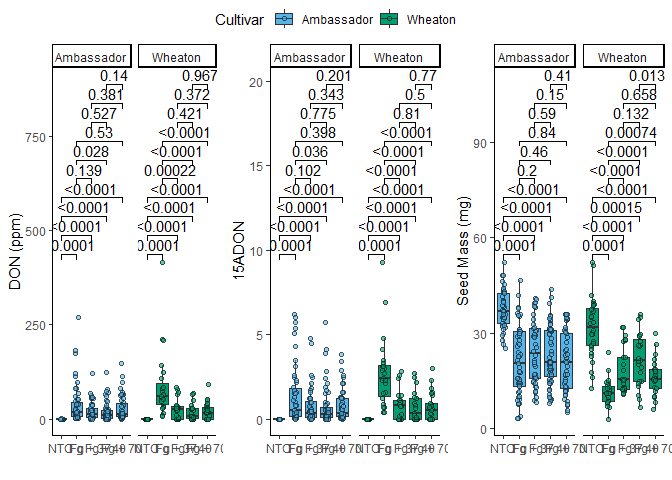
\includegraphics{R-markdown-coding-challange_files/figure-latex/unnamed-chunk-5-1.pdf}

\end{document}
